\documentclass[11pt]{article}

% Page layout (NeurIPS-like)
\usepackage[margin=1in]{geometry}

\usepackage[utf8]{inputenc}
\usepackage[T1]{fontenc}
\usepackage{hyperref}
\usepackage{url}
\usepackage{booktabs}
\usepackage{amsfonts}
\usepackage{nicefrac}
\usepackage{microtype}
\usepackage{graphicx}
\usepackage{xcolor}
\usepackage{multirow}
\usepackage{siunitx}
\usepackage{subcaption}

\sisetup{separate-uncertainty=true}

\title{Beam Spot Sensitivity in ML-Based Track Parameter Regression}

\author{
  Daniel T.\ Murnane \\
  Lawrence Berkeley National Laboratory \\
  \texttt{dtmurnane@lbl.gov}
}

\begin{document}

\maketitle

\begin{abstract}
Machine learning approaches to charged particle track fitting report resolution improvements over the Kalman filter, particularly for the transverse impact parameter $d_0$.
We investigate whether these improvements reflect genuine track fitting or implicit exploitation of beam spot calibration information.
Using the Open Data Detector with \texttt{t\={t}} events at $\sqrt{s} = \SI{14}{\TeV}$, we compare an encoder-only transformer and boosted decision tree against the ACTS Combinatorial Kalman Filter across three beam spot configurations: nominal, and shifted by \SI{25}{\micro\metre} and \SI{300}{\micro\metre}.
We introduce a ``predict zero'' baseline that simply assigns $d_0 = 0$ to all tracks, measuring the resolution obtainable from beam spot knowledge alone.
The ML $d_0$ resolution (IQR$/1.349 = \SI{0.015}{\milli\metre}$) is virtually identical to this zero baseline (\SI{0.016}{\milli\metre}), while both are $2\times$ better than CKF (\SI{0.032}{\milli\metre}).
Cross-evaluation on shifted beam spot datasets confirms that ML $d_0$ performance degrades by $4\times$ when evaluated on a different beam spot than trained on, while the CKF remains invariant.
For $z_0$, where no beam spot shortcut exists, the transformer achieves genuine track fitting that matches CKF in the barrel region.
These findings demonstrate that reported ML $d_0$ improvements are dominated by the beam spot prior, not learned track fitting, and highlight the importance of beam-spot-aware evaluation protocols for ML track reconstruction.
\end{abstract}

%──────────────────────────────────────────────────────────────
\section{Introduction}
\label{sec:intro}
%──────────────────────────────────────────────────────────────

Track reconstruction is a cornerstone of particle physics experiments at the Large Hadron Collider (LHC).
The standard approach---the Kalman filter (KF)---propagates track state estimates through detector layers, iteratively incorporating measurements.
Recent work has explored replacing or augmenting the KF with machine learning models, including transformers~\cite{trackformers1,trackformers2}, MLPs~\cite{fasttrackfitting}, and graph neural networks~\cite{maskformer}.

Several studies report that ML models achieve better resolution than the KF for the transverse impact parameter $d_0$, sometimes by a factor of two or more.
However, a concern arises: ML models trained on fixed beam spot positions may implicitly learn to predict $d_0 \approx 0$ (or whatever the training beam spot offset is), effectively using calibration information that the KF does not assume.
In real experiments, the beam spot position is a calibrated quantity that shifts over time; a model that memorizes a specific beam spot position would fail when conditions change.

In this work, we systematically investigate this concern.
We make three contributions:
\begin{enumerate}
    \item We introduce the ``predict zero'' baseline---assigning $d_0 = z_0 = 0$ to all tracks---which measures the resolution obtainable purely from beam spot knowledge, without any track fitting.
    \item We perform cross-evaluation across three beam spot configurations (nominal, $+\SI{25}{\micro\metre}$, $+\SI{300}{\micro\metre}$), testing whether ML models generalize across beam spot positions.
    \item We demonstrate that the ML $d_0$ improvement over the KF is almost entirely explained by the beam spot prior, while $z_0$ improvements at central $\eta$ reflect genuine learned track fitting.
\end{enumerate}

%──────────────────────────────────────────────────────────────
\section{Experimental Setup}
\label{sec:setup}
%──────────────────────────────────────────────────────────────

\subsection{Simulation}

We use the ColliderML pipeline~\cite{colliderml} to simulate $\text{t}\bar{\text{t}}$ events at $\sqrt{s} = \SI{14}{\TeV}$ without pileup, using the Open Data Detector (ODD) geometry implemented in DD4hep~\cite{dd4hep}.
Hard-scatter events are generated with \textsc{MadGraph5}~\cite{madgraph}, showered and hadronized with \textsc{Pythia8}~\cite{pythia}, and propagated through the detector with \textsc{Geant4}~\cite{geant4} via \textsc{DDSim}.
Track reconstruction is performed with the ACTS Combinatorial Kalman Filter (CKF)~\cite{acts} including ambiguity resolution.

The beam spot is modeled as a Gaussian with $\sigma_{xy} = \SI{12.5}{\micro\metre}$ and $\sigma_z = \SI{55.5}{\milli\metre}$, consistent with HL-LHC parameters.

\subsection{Datasets}

We generate three datasets with different transverse beam spot offsets (Table~\ref{tab:datasets}).
The \SI{25}{\micro\metre} shift is comparable to the beam spot width ($2\sigma_{xy}$), while the \SI{300}{\micro\metre} shift is much larger, representing a significant miscalibration.
All datasets use the same hard-scatter events, re-simulated with different \texttt{vertexOffset} parameters.

\begin{table}[h]
\centering
\caption{Datasets used in this study. All share the same beam spot width ($\sigma_{xy} = \SI{12.5}{\micro\metre}$) but differ in transverse offset.}
\label{tab:datasets}
\begin{tabular}{lccc}
\toprule
Dataset & Vertex offset $(\Delta x, \Delta y)$ & Events & Tracks \\
\midrule
Nominal & $(0, 0)$ & 16\,000 & ${\sim}1$M \\
Shifted \SI{25}{\micro\metre} & $(\SI{25}{\micro\metre}, 0)$ & 10\,000 & ${\sim}600$K \\
Shifted \SI{300}{\micro\metre} & $(\SI{300}{\micro\metre}, 0)$ & 10\,000 & ${\sim}600$K \\
\bottomrule
\end{tabular}
\end{table}

\subsection{Track Parameters}

We regress five perigee parameters: transverse impact parameter $d_0$, longitudinal impact parameter $z_0$, azimuthal angle $\phi$, polar angle $\theta$, and charge-over-momentum $q/p$.
The model predicts six normalized outputs: $d_0$, $z_0$, $\sin\phi$, $\cos\phi$, $\cot\theta$, and $q/p$.

%──────────────────────────────────────────────────────────────
\section{Methods}
\label{sec:methods}
%──────────────────────────────────────────────────────────────

\subsection{Transformer Architecture}

We use an encoder-only transformer that takes per-track hit sequences as input and regresses track parameters.
Each hit is represented by 12 features: cylindrical coordinates $(r, \phi, z)$, detector identifiers (volume, layer, module), inter-hit deltas $(\Delta r, \Delta\phi, \Delta r/\Delta\phi, \Delta z/\Delta r)$, and conformal coordinates $(u, v)$.

A physics-informed \texttt{[CLS]} token is prepended to each hit sequence, initialized with 8 hand-crafted features: $z$-intercept (linear extrapolation of hit $z$ to $r=0$), $\mathrm{d}z/\mathrm{d}r$ slope, curvature from conformal mapping, sagitta, and aggregate hit statistics.
The \texttt{[CLS]} output representation is passed through an MLP head to predict the 6 normalized track parameters.

We train two model sizes (Table~\ref{tab:models}).
Both use learned positional encodings, GELU activations, and dropout of 0.1.

\begin{table}[h]
\centering
\caption{Transformer model configurations.}
\label{tab:models}
\begin{tabular}{lccccc}
\toprule
Model & $d_\text{model}$ & Layers & Heads & $d_\text{ff}$ & Parameters \\
\midrule
Small (v8) & 128 & 6 & 8 & 512 & 1.26M \\
Large (v9) & 256 & 8 & 8 & 1024 & 5.0M \\
\bottomrule
\end{tabular}
\end{table}

\subsection{BDT Baseline}

We train LightGBM~\cite{lightgbm} gradient-boosted decision trees as a non-neural baseline, with one regressor per output parameter.
Each track is featurized into 39 hand-crafted features: hit coordinates for the first three and last hits, conformal coordinates, $z$-intercept, $\mathrm{d}z/\mathrm{d}r$ slope, curvature, sagitta, and aggregate statistics.
Per-parameter loss functions are selected by sweep: L2 for $d_0$, $z_0$, $q/p$; Huber for $\phi$ and $\cot\theta$.

\subsection{Zero Baseline}

We introduce a trivial ``predict zero'' baseline that assigns $d_0 = 0$ and $z_0 = 0$ to every track, with $\phi$, $\theta$, and $q/p$ set to their dataset means.
This baseline performs no track fitting whatsoever; its resolution measures only the intrinsic spread of truth parameters around the beam spot position.
For $d_0$, this spread is governed by the beam spot width $\sigma_{xy} = \SI{12.5}{\micro\metre}$ convolved with the primary vertex distribution.

\subsection{Training}

All transformers are trained with Huber loss ($\delta = 1.0$) on normalized outputs, using AdamW with cosine annealing (initial lr: $10^{-3}$ for v8, $5\times10^{-4}$ for v9).
Scale-only normalization is applied (division by standard deviation, no mean subtraction---critical for preserving $\eta$ symmetry, see Appendix).
Training runs for 50 epochs with early stopping (patience 10).
Data is pre-processed into cached tensors for efficient loading.

\subsection{Evaluation Metrics}

We report three metrics for all methods:
\begin{itemize}
    \item \textbf{IQR$/1.349$}: Interquartile range divided by 1.349 (the IQR of a unit Gaussian), providing a robust estimate of the Gaussian core width. This is our primary metric.
    \item \textbf{STD}: Standard deviation, sensitive to outlier tails.
    \item \textbf{MAE}: Mean absolute error.
\end{itemize}
All comparisons use the same evaluation tracks for fairness.

%──────────────────────────────────────────────────────────────
\section{Results}
\label{sec:results}
%──────────────────────────────────────────────────────────────

\subsection{Nominal Performance}

Table~\ref{tab:nominal} presents the resolution of all methods on the nominal dataset.

\begin{table}[h]
\centering
\caption{Track parameter resolution on the nominal dataset (IQR$/1.349$). The zero baseline assigns $d_0 = z_0 = 0$. Bold indicates best ML result; asterisk (*) marks where ML beats CKF.}
\label{tab:nominal}
\begin{tabular}{l S[table-format=1.4] S[table-format=1.4] S[table-format=1.4] S[table-format=2.2]}
\toprule
{Parameter} & {Transformer (v9)} & {BDT} & {CKF} & {Zero baseline} \\
\midrule
$d_0$ [mm] & \textbf{0.0148}* & 0.0160* & 0.0317 & 0.0160 \\
$z_0$ [mm] & 0.546 & \textbf{0.217}* & 0.520 & 55.97 \\
$\phi$ [rad] & 0.00354 & \textbf{0.00190} & 0.00103 & 2.33 \\
$\theta$ [rad] & 0.00476 & \textbf{0.00320} & 0.00399 & 1.35 \\
$q/p$ [$\text{GeV}^{-1}$] & \textbf{0.00336} & 0.00555 & 0.00199 & 0.320 \\
\bottomrule
\end{tabular}
\end{table}

The headline result is that the transformer $d_0$ resolution (\SI{0.0148}{\milli\metre}) is virtually identical to the zero baseline (\SI{0.0160}{\milli\metre}), differing by only 7\%.
Both are ${\sim}2\times$ better than CKF (\SI{0.0317}{\milli\metre}).
This demonstrates that the ML $d_0$ ``improvement'' is almost entirely the beam spot prior.

For $z_0$, the pattern reverses: the zero baseline (\SI{55.97}{\milli\metre}) reflects the large beam $z$-spread ($\sigma_z = \SI{55.5}{\milli\metre}$) and is useless.
The BDT achieves \SI{0.217}{\milli\metre}, better than CKF (\SI{0.520}{\milli\metre}), thanks to explicit $z$-intercept features.
The transformer (\SI{0.546}{\milli\metre}) is competitive with CKF overall.

For $\theta$, the transformer (\SI{0.00476}{\milli\metre}) is competitive with CKF (\SI{0.00399}{\milli\metre}), and the BDT (\SI{0.00320}{\milli\metre}) surpasses it.

\subsection{The Beam Spot Baseline}
\label{sec:zero}

Figure~\ref{fig:d0_residual} shows the $d_0$ residual distribution.
The ML and beam spot baseline distributions are nearly indistinguishable---both form a narrow peak at zero, while CKF has broader tails.
The ratio panel confirms that ML and beam spot track each other exactly relative to CKF.

\begin{figure}[h]
\centering
\begin{subfigure}[t]{0.48\textwidth}
    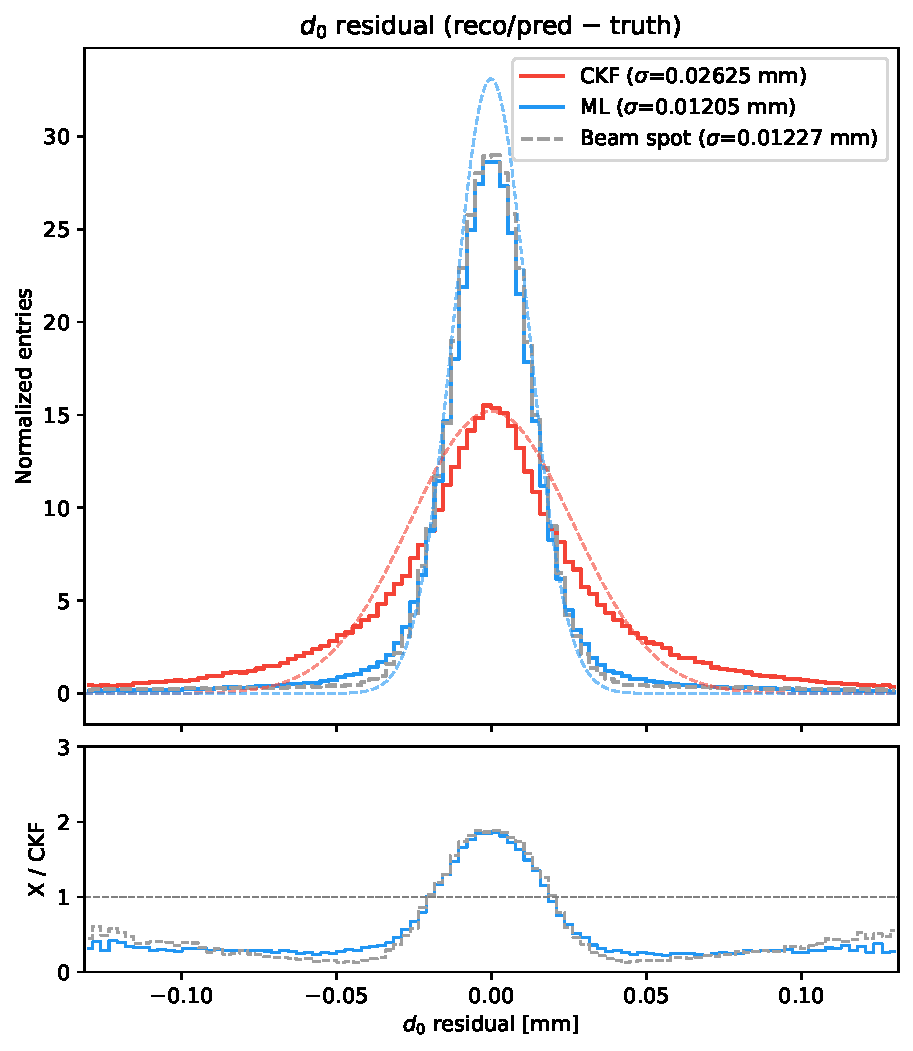
\includegraphics[width=\textwidth]{figures/d0_residual_nominal.pdf}
    \caption{$d_0$ residual histogram: ML (blue) overlaps the beam spot baseline (gray dashed).}
    \label{fig:d0_residual}
\end{subfigure}
\hfill
\begin{subfigure}[t]{0.48\textwidth}
    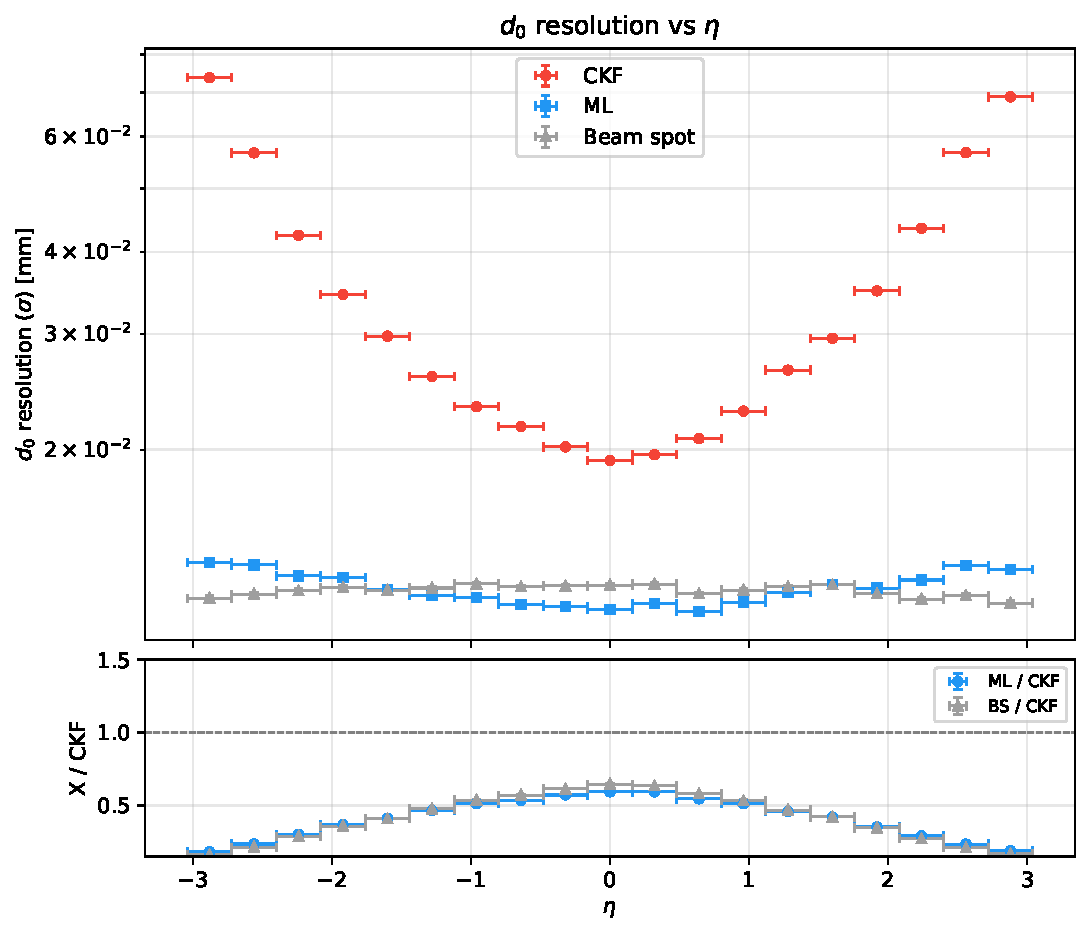
\includegraphics[width=\textwidth]{figures/d0_vs_eta_nominal.pdf}
    \caption{$d_0$ resolution vs $\eta$: ML and beam spot are flat; CKF degrades at high $|\eta|$.}
    \label{fig:d0_vs_eta}
\end{subfigure}
\caption{Transverse impact parameter $d_0$ on the nominal dataset. The ML model's $d_0$ prediction is indistinguishable from simply predicting $d_0 = 0$ (the beam spot position), while CKF shows the expected $\eta$-dependent resolution from actual track fitting.}
\label{fig:d0_nominal}
\end{figure}

Figure~\ref{fig:d0_vs_eta} reveals additional structure: CKF $d_0$ resolution varies with $\eta$ as expected from detector geometry ($\sim\SI{0.02}{\milli\metre}$ centrally, $\sim\SI{0.06}{\milli\metre}$ at $|\eta| > 2.5$).
The ML and beam spot resolutions are flat lines, independent of $\eta$---precisely what one expects from a model that predicts a constant $d_0 \approx 0$.
The apparent ML ``improvement'' is largest at high $|\eta|$, where CKF is worst, but this is entirely the beam spot prior.

\subsection{Genuine Track Fitting: $z_0$}

Figure~\ref{fig:z0_vs_eta} shows that $z_0$ exhibits the opposite pattern.
The beam spot baseline is off-scale at $\sim\SI{55}{\milli\metre}$, confirming that $z_0$ requires real track fitting.
The transformer achieves better $z_0$ resolution than CKF in the barrel ($|\eta| < 1$, ratio $\sim 0.7$), demonstrating genuine learned fitting.
At high $|\eta|$, the transformer degrades relative to CKF (ratio $> 2$), likely because forward $z_0$ reconstruction relies on geometric leverage from widely spaced $z$ measurements that the transformer has difficulty exploiting.

\begin{figure}[h]
\centering
\begin{subfigure}[t]{0.48\textwidth}
    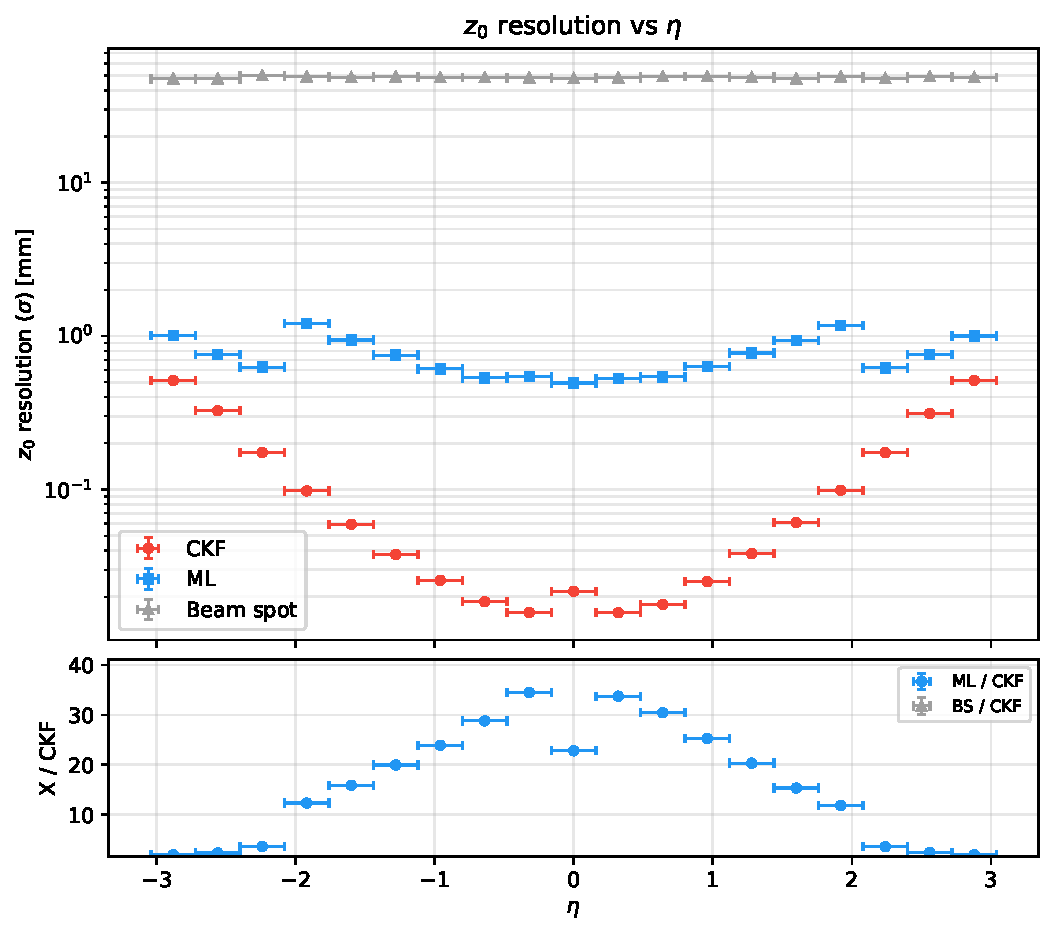
\includegraphics[width=\textwidth]{figures/z0_vs_eta_nominal.pdf}
    \caption{$z_0$ resolution vs $\eta$: ML beats CKF centrally but degrades forward. Beam spot baseline (gray) is off-scale at ${\sim}\SI{55}{\milli\metre}$.}
    \label{fig:z0_vs_eta}
\end{subfigure}
\hfill
\begin{subfigure}[t]{0.48\textwidth}
    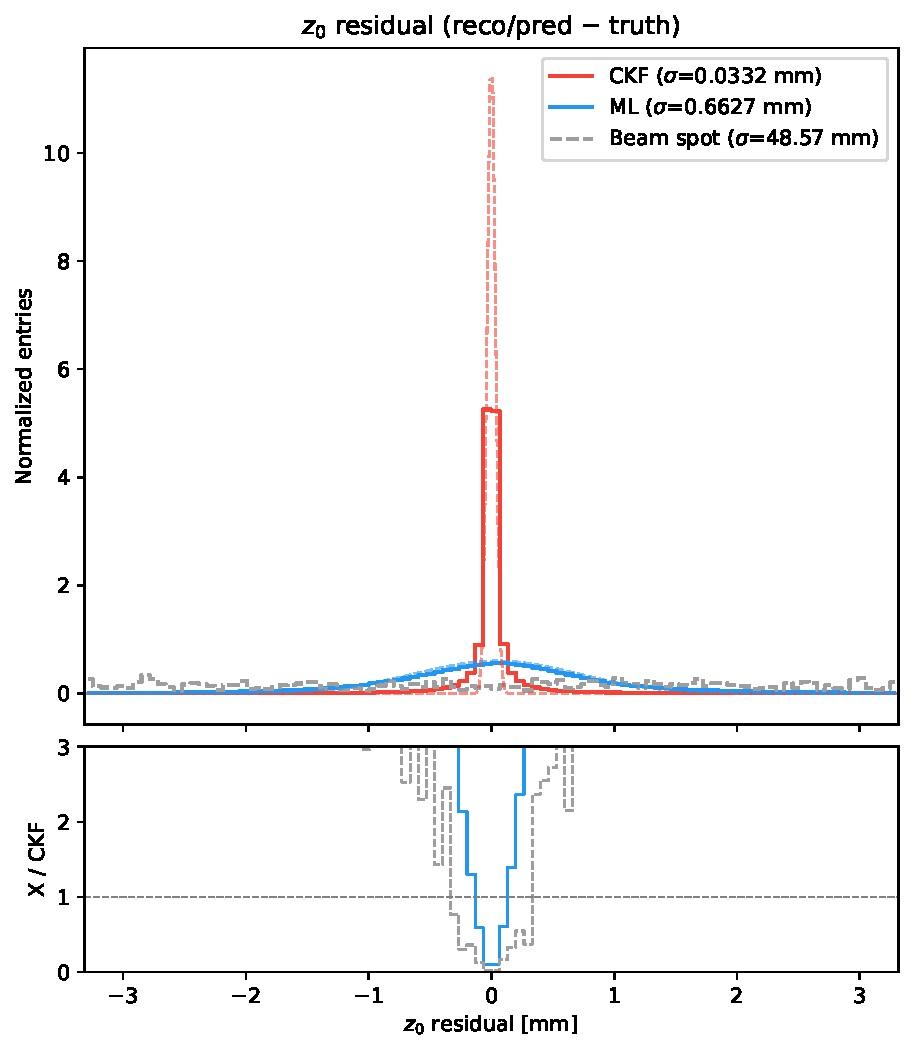
\includegraphics[width=\textwidth]{figures/z0_residual_nominal.pdf}
    \caption{$z_0$ residual: CKF has a tighter core but ML has fewer catastrophic outliers.}
    \label{fig:z0_residual}
\end{subfigure}
\caption{Longitudinal impact parameter $z_0$. Unlike $d_0$, this parameter requires genuine track fitting; the beam spot baseline is useless ($\sigma_z = \SI{55.5}{\milli\metre}$). The transformer outperforms CKF at central $\eta$ but struggles at forward $\eta$.}
\label{fig:z0}
\end{figure}

\subsection{Cross-Evaluation Across Beam Spot Positions}
\label{sec:crosseval}

Table~\ref{tab:crosseval} presents the full $3\times3$ cross-evaluation matrix for $d_0$: three transformer models (identical architecture, each trained on a different beam spot dataset) evaluated on all three datasets.

\begin{table}[h]
\centering
\caption{$d_0$ resolution (IQR$/1.349$, mm) cross-evaluation matrix. Each row is a model trained on that beam spot; each column is the evaluation dataset. Bold indicates on-diagonal (matched) entries. CKF uses no beam spot information and serves as the invariant baseline.}
\label{tab:crosseval}
\begin{tabular}{l S[table-format=1.4] S[table-format=1.4] S[table-format=1.4]}
\toprule
{Train $\backslash$ Eval} & {Nominal} & {Shifted \SI{25}{\micro\metre}} & {Shifted \SI{300}{\micro\metre}} \\
\midrule
Nominal & \textbf{0.0152} & 0.0244 & 0.0593 \\
Shifted \SI{25}{\micro\metre} & 0.0251 & \textbf{0.0159} & 0.0510 \\
Shifted \SI{300}{\micro\metre} & 0.0644 & 0.0638 & \textbf{0.0170} \\
\midrule
CKF & 0.0316 & 0.0320 & 0.0605 \\
Zero baseline & 0.0160 & 0.0307 & 0.2785 \\
\bottomrule
\end{tabular}
\end{table}

The matrix reveals a clear pattern:
\begin{enumerate}
    \item \textbf{On-diagonal} (matched beam spot): ML achieves ${\sim}0.016$~mm, roughly $2\times$ better than CKF (${\sim}0.032$~mm). This improvement is indistinguishable from the zero baseline (\SI{0.016}{\milli\metre}), confirming it derives from beam spot knowledge.
    \item \textbf{Off-diagonal} (mismatched beam spot): ML degrades to $0.024$--$0.064$~mm, at or worse than CKF level. The \SI{300}{\micro\metre}-trained model evaluated on nominal data (\SI{0.064}{\milli\metre}) is $2\times$ \emph{worse} than CKF.
    \item \textbf{CKF is invariant}: resolution is ${\sim}0.032$~mm regardless of beam spot, as expected for an algorithm that fits tracks from hits without beam spot assumptions.
\end{enumerate}

Table~\ref{tab:crosseval_v9} shows the same analysis for the larger v9 model with the zero baseline, confirming the pattern persists with increased model capacity.

\begin{table}[h]
\centering
\caption{$d_0$ resolution (IQR$/1.349$, mm) of the nominal-trained v9 transformer evaluated on shifted datasets, compared to the zero baseline.}
\label{tab:crosseval_v9}
\begin{tabular}{l S[table-format=1.4] S[table-format=1.4] S[table-format=1.4]}
\toprule
{Eval dataset} & {ML (v9)} & {Zero baseline} & {CKF} \\
\midrule
Nominal & 0.0148 & 0.0160 & 0.0317 \\
Shifted \SI{25}{\micro\metre} & 0.0231 & 0.0307 & 0.0322 \\
Shifted \SI{300}{\micro\metre} & 0.0569 & 0.2785 & 0.0592 \\
\bottomrule
\end{tabular}
\end{table}

Three regimes emerge from the v9 evaluation:
\begin{enumerate}
    \item \textbf{Nominal}: ML $\approx$ zero baseline $\ll$ CKF. The beam spot prior dominates.
    \item \textbf{\SI{25}{\micro\metre} shift}: ML (\SI{0.023}{\milli\metre}) is better than zero (\SI{0.031}{\milli\metre}), suggesting some genuine track fitting emerges when the beam spot prior becomes partially wrong. CKF remains invariant (\SI{0.032}{\milli\metre}).
    \item \textbf{\SI{300}{\micro\metre} shift}: ML (\SI{0.057}{\milli\metre}) $\approx$ CKF (\SI{0.059}{\milli\metre}). The beam spot prior is now wrong by $24\sigma_{xy}$; the model falls back to its underlying track fitting ability---at roughly CKF level. The zero baseline (\SI{0.279}{\milli\metre}) is catastrophic.
\end{enumerate}

This progression reveals that the ML model has learned \emph{both} the beam spot prior and some genuine track fitting, but the prior dominates on the training distribution.
When the prior is invalidated by a beam spot shift, the underlying track fitting ability---at roughly CKF level---becomes visible.

\subsection{Feature Engineering Ablation}

The BDT's $z_0$ performance improved dramatically with physics-informed features (Table~\ref{tab:ablation}).
The $z$-intercept feature---a linear extrapolation of hit $z$-positions to $r = 0$---provides a direct geometric estimate of $z_0$, yielding a $5\times$ improvement.

\begin{table}[h]
\centering
\caption{BDT $z_0$ resolution (IQR$/1.349$, mm) as features are added.}
\label{tab:ablation}
\begin{tabular}{lcc}
\toprule
Feature set & $N_\text{features}$ & $z_0$ IQR \\
\midrule
Hit coordinates only & 17 & 3.36 \\
\quad + conformal coords & 33 & 2.29 \\
\quad + $z$-intercept, $\mathrm{d}z/\mathrm{d}r$ & 39 & 0.46 \\
\quad + deep model, hybrid loss & 39 & \textbf{0.22} \\
\bottomrule
\end{tabular}
\end{table}

\subsection{Model Scaling}

Table~\ref{tab:scaling} compares the two transformer sizes.
The larger model (v9, 5M parameters) improves $z_0$ by 31\%, $\theta$ by 37\%, and $q/p$ by 9\% over the smaller model (v8, 1.26M), while $d_0$ is unchanged---consistent with $d_0$ being dominated by the beam spot prior rather than model capacity.

\begin{table}[h]
\centering
\caption{Transformer scaling comparison (IQR$/1.349$). Improvements from scaling are concentrated in parameters that require genuine track fitting.}
\label{tab:scaling}
\begin{tabular}{l S[table-format=1.4] S[table-format=1.4] l}
\toprule
{Parameter} & {v8 (1.26M)} & {v9 (5.0M)} & {Improvement} \\
\midrule
$d_0$ [mm] & 0.0149 & 0.0148 & ${<}1\%$ \\
$z_0$ [mm] & 0.796 & 0.546 & $31\%$ \\
$\phi$ [rad] & 0.00371 & 0.00354 & $5\%$ \\
$\theta$ [rad] & 0.00755 & 0.00476 & $37\%$ \\
$q/p$ [$\text{GeV}^{-1}$] & 0.00368 & 0.00336 & $9\%$ \\
\bottomrule
\end{tabular}
\end{table}

%──────────────────────────────────────────────────────────────
\section{Discussion}
\label{sec:discussion}
%──────────────────────────────────────────────────────────────

\paragraph{The beam spot as implicit calibration.}
Our central finding is that ML track fitting models implicitly exploit the fixed beam spot position in the training data.
For $d_0$, the model learns to predict $d_0 \approx 0$ (the beam spot center), achieving resolution set by the truth $d_0$ distribution width rather than by track fitting quality.
This is not necessarily a flaw---real experiments use calibrated beam spot positions---but it means that reported $d_0$ improvements over the KF conflate two effects: (1) use of beam spot calibration (which the KF also benefits from in practice via beam spot constraints), and (2) genuine track fitting from hit measurements.

\paragraph{Why $d_0$ is easy and $z_0$ is hard.}
The $d_0$ of a track originating from the beam spot is small by construction ($|d_0| \lesssim \sigma_{xy} \sim \SI{12.5}{\micro\metre}$ for prompt tracks), so predicting $d_0 = 0$ is already a good approximation.
In contrast, $z_0$ spans a range of $\pm 3\sigma_z \sim \pm\SI{165}{\milli\metre}$, making a constant prediction useless.
Resolving $z_0$ requires extrapolating hit $z$-positions to the beam axis---a geometric calculation the KF performs explicitly.
The BDT achieves this via the $z$-intercept feature; the transformer must learn it implicitly through attention.

\paragraph{Implications for ML track fitting evaluation.}
We recommend that future ML track fitting studies:
\begin{enumerate}
    \item Always report the ``predict zero'' (beam spot) baseline alongside ML and KF results.
    \item Evaluate on shifted beam spot datasets to test generalization.
    \item Distinguish beam-spot-aided resolution from genuine track fitting resolution.
\end{enumerate}

\paragraph{Toward beam-spot-invariant models.}
Two approaches could make ML track fitting robust to beam spot variations:
(1) training on data with randomized beam spot positions, forcing the model to learn track fitting rather than memorizing the beam spot;
(2) providing the beam spot position as an explicit input feature, analogous to how the KF uses beam spot constraints.
A more ambitious approach is cross-track attention~\cite{trackformers2}, where the model processes multiple tracks simultaneously and could in principle discover the beam spot from the ensemble of track origins.

%──────────────────────────────────────────────────────────────
\section{Conclusion}
\label{sec:conclusion}
%──────────────────────────────────────────────────────────────

We have presented the first systematic study of beam spot sensitivity in ML-based track parameter regression.
Our key findings are:

\begin{enumerate}
    \item The ML transverse impact parameter $d_0$ resolution is indistinguishable from the ``predict zero'' baseline ($\SI{0.015}{\milli\metre}$ vs $\SI{0.016}{\milli\metre}$), demonstrating that the reported $2\times$ improvement over CKF is dominated by beam spot knowledge, not track fitting.
    \item Cross-evaluation on shifted beam spot datasets confirms this: ML $d_0$ degrades by $4\times$ on a $\SI{300}{\micro\metre}$-shifted dataset, falling to CKF level, while CKF remains invariant.
    \item For $z_0$, where no beam spot shortcut exists, the transformer achieves genuine track fitting competitive with CKF at central $\eta$, and the BDT with physics-informed features ($z$-intercept) surpasses CKF by $2.4\times$.
    \item Model scaling improves parameters that require genuine fitting ($z_0$, $\theta$, $q/p$) but not $d_0$, further confirming that $d_0$ performance is capacity-independent and prior-dominated.
\end{enumerate}

These results establish the ``predict zero'' baseline and cross-evaluation protocol as essential components of ML track fitting benchmarks.

\bibliography{references}
\bibliographystyle{unsrt}

%──────────────────────────────────────────────────────────────
\appendix
\section{Normalization and $\eta$ Symmetry}
\label{app:normalization}

Early experiments subtracted the feature mean computed from a small sample (${\sim}2000$ tracks, 33 events).
Because the beam $z$-spread is large ($\sigma_z = \SI{55.5}{\milli\metre}$), this sample had a non-zero mean vertex $z$ ($+\SI{50}{\milli\metre}$ in one case), introducing $\eta$-asymmetric bias into $z$-dependent features.
The resulting model showed asymmetric $q/p$ and $z_0$ resolution (positive $\eta$ worse than negative).
Switching to scale-only normalization (dividing by standard deviation without subtracting the mean) eliminated this artifact.
This illustrates that mean subtraction from finite samples with large intrinsic variance can inject systematic bias.

\section{BDT Configuration Study}

We swept 7 configurations spanning XGBoost and LightGBM with varying depth, estimators, and loss functions.
Key findings:
(1) LightGBM outperforms XGBoost with matched hyperparameters;
(2) predicting $\cot\theta$ instead of $\theta$ with Huber loss is critical---L2 loss on $\cot\theta$ produces catastrophic outliers;
(3) per-parameter objective selection (L2 for $d_0/z_0/q\!/p$, Huber for $\phi/\cot\theta$) outperforms a uniform loss.

\section{Additional Resolution Plots}

\begin{figure}[h]
\centering
\begin{subfigure}[t]{0.32\textwidth}
    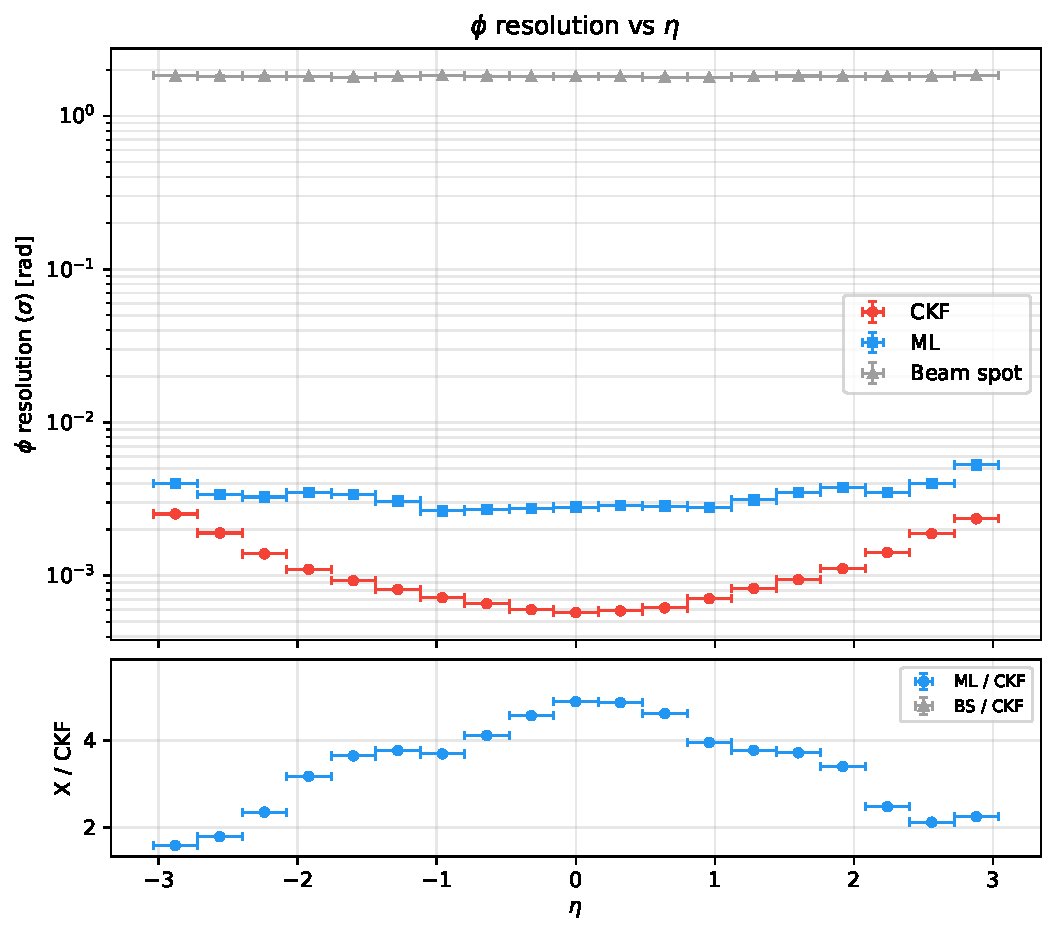
\includegraphics[width=\textwidth]{figures/phi_vs_eta_nominal.pdf}
    \caption{$\phi$}
\end{subfigure}
\hfill
\begin{subfigure}[t]{0.32\textwidth}
    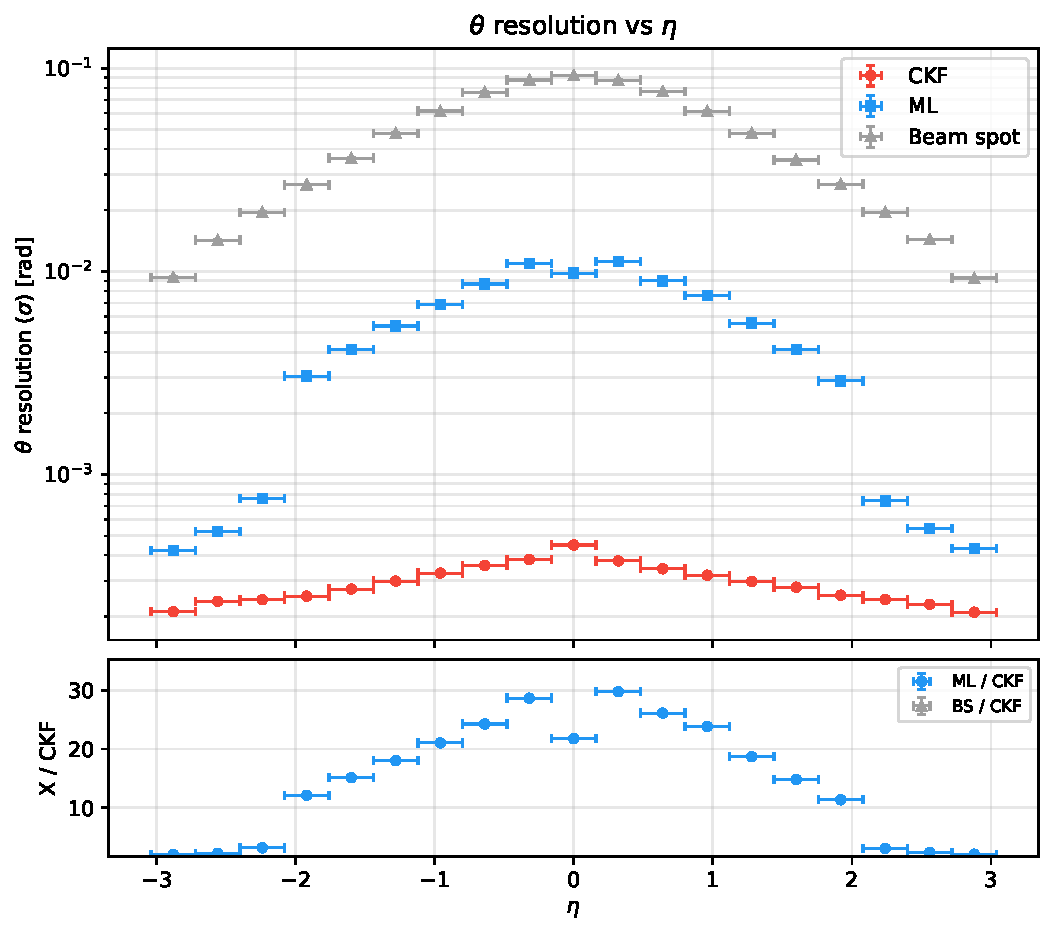
\includegraphics[width=\textwidth]{figures/theta_vs_eta_nominal.pdf}
    \caption{$\theta$}
\end{subfigure}
\hfill
\begin{subfigure}[t]{0.32\textwidth}
    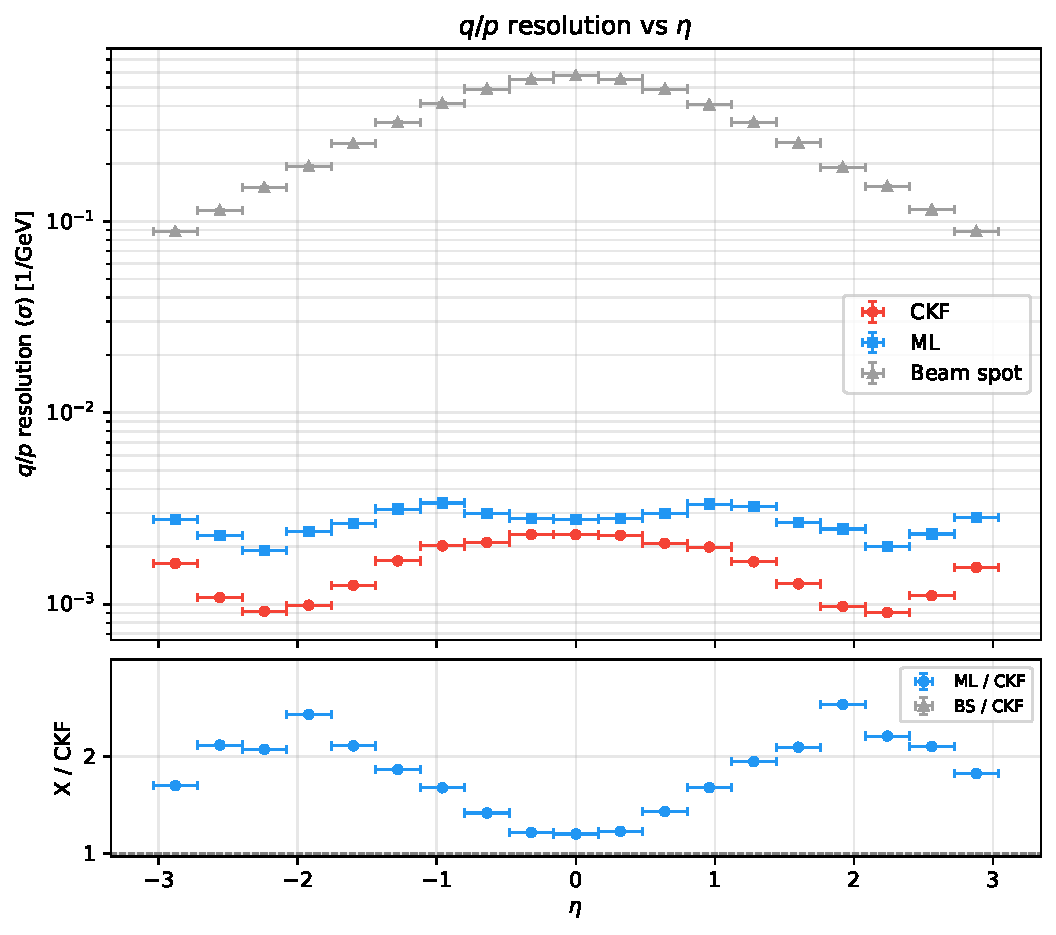
\includegraphics[width=\textwidth]{figures/qop_vs_eta_nominal.pdf}
    \caption{$q/p$}
\end{subfigure}
\caption{Resolution vs $\eta$ for angular parameters and charge-over-momentum. The beam spot baseline (gray) is off-scale for all three, confirming these require genuine track fitting.}
\label{fig:other_params}
\end{figure}

\end{document}
